% ---------------------------------------------------------------------------- %
\begin{figure}
  \centering
	\subfigure[\label{fig:results:uovo:aln:before}]
	{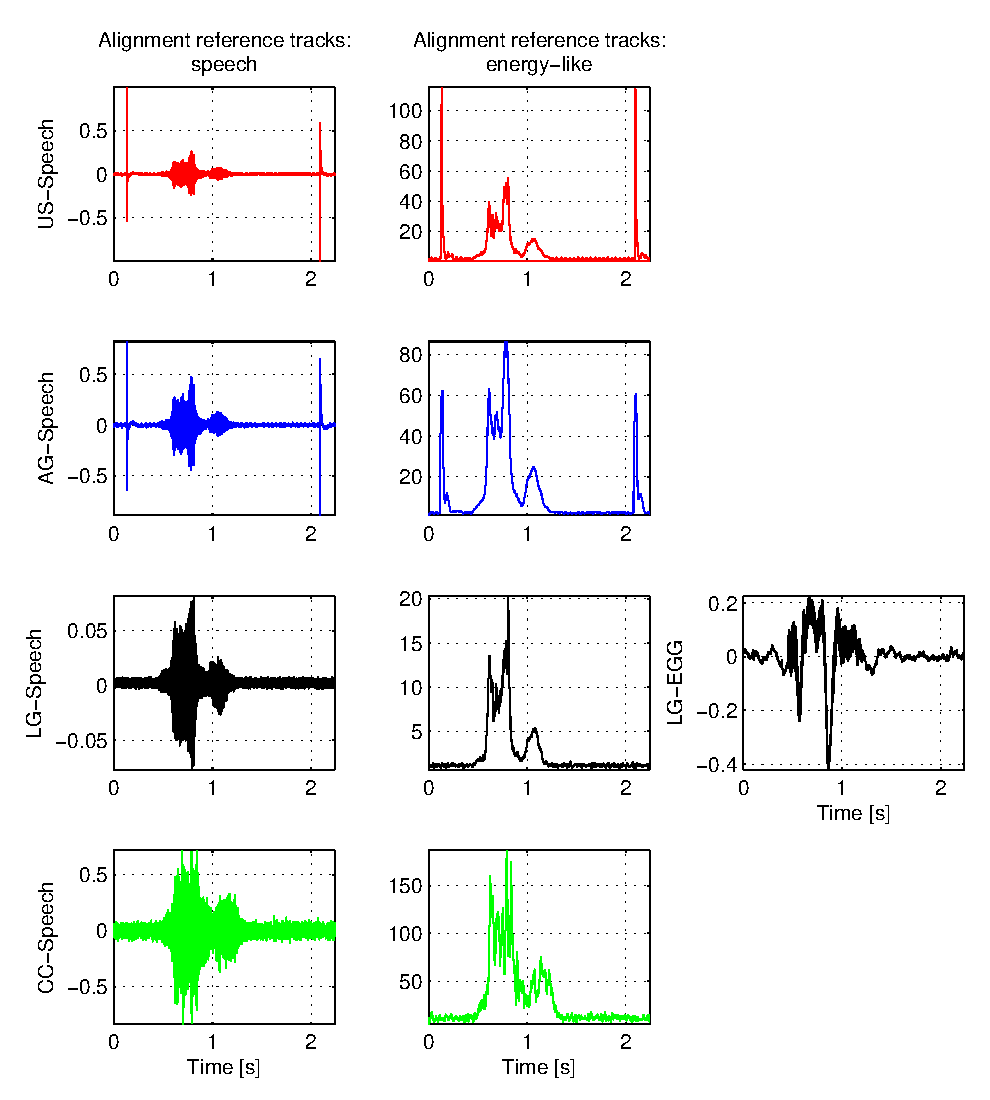
\includegraphics[width=0.45\textwidth]{include/results/images/final_15_before.eps}}
	\hspace{0.05\textwidth}
	\subfigure[\label{fig:results:uovo:aln:after}]
	{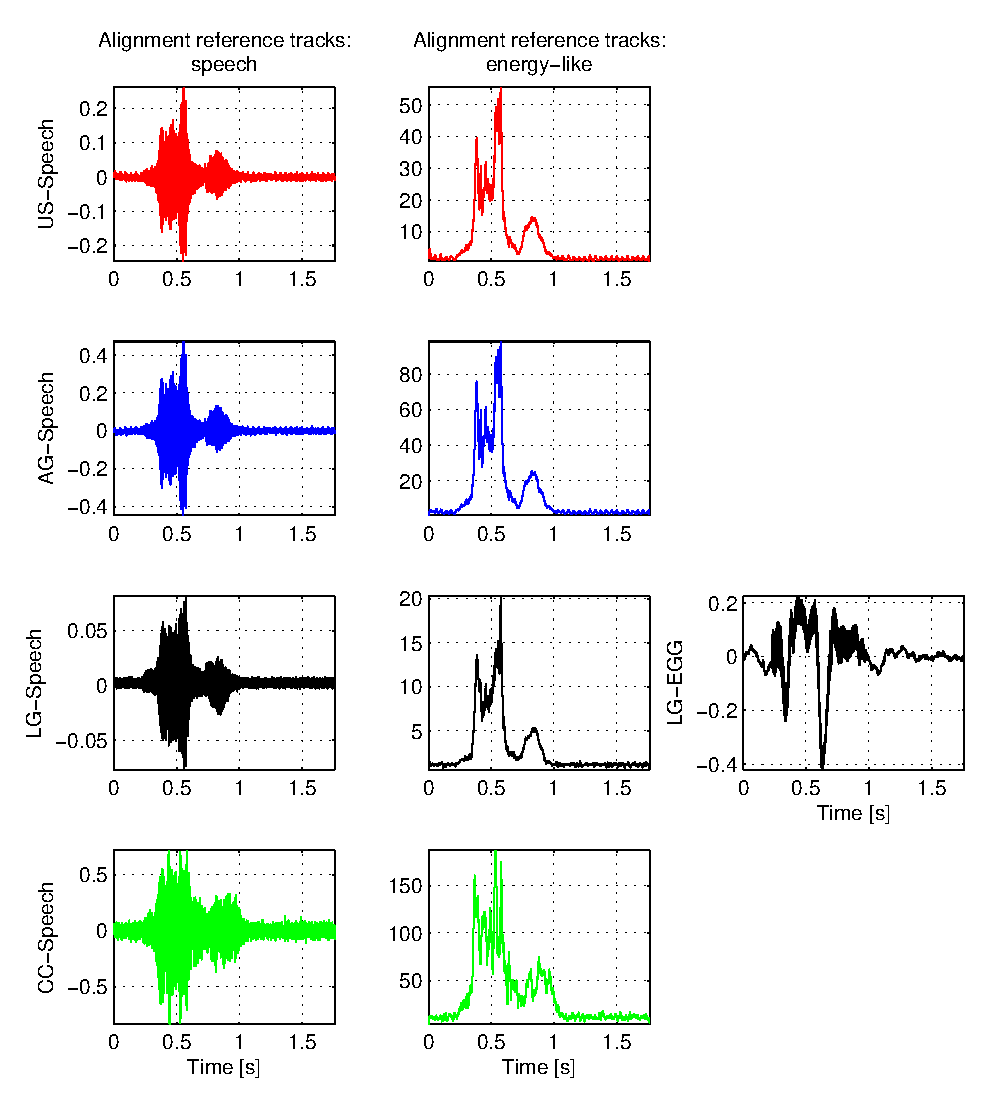
\includegraphics[width=0.45\textwidth]{include/results/images/final_15_after.eps}}

	\caption[Alignment results for /uovo/]{\textbf{Alignment
	results for /uovo/}: 
	The \wf{US-Speech} signal is used as reference during the alignment via the
	{\tt lm\_packages} Perl script.
	As P. Fitzpatrick initially suggested, the alignment is performed by
	the means of cross-correlation between ``energy-like'' signals.
	Those last signals correspond to a smoothed version of the absolute values
	of the speech signals.
	The data before alignment is shown in (a), while (b) shows the same signals
	after alignment.
	For each panel, the energy-like signals are shown. 
	Before performing the alignment procedure, the segmentation 
	peaks are removed from \wf{US-Speech} and \wf{AG-Speech}. In fact, the
	segmentation peaks visible in (a) are not visible in the final alignment 
	results (b).
	No information  about \wf{US-Video} or \wf{CC-Video} is shown, since the
	feature extraction algorithms are still under development.
	Furthermore, the \wf{AG-AMP} and the \wf{AG-POS} data are not shown in this
	Figure due their multi-dimensional nature.
	}
	\label{fig:results:uovo:aln}
\end{figure}
% ---------------------------------------------------------------------------- %
